\chapter{Appendix}
\label{app:appendix_A}
The appendix roughly follows the structure of the main thesis. Some of the tables and plots from the intermediate experiments section (Appendix \ref{sec:appendix_A3}) were obtained during an exploratory phase and thus are only approximated and do not contain subject-wise information. However they should give an overview of the logical reasoning that led to the final experiment, for which more individual information is reported in Appendix \ref{sec:appendix_A4}. Individual ROC curves, labels distribution and confusion matrices are only reported for specific examples regarding the unbalance of some datasets (see Appendix \ref{sec:appendix_A3.3})

\section{Pilot study}
\label{sec:appendix_A1}
A pilot study was run internally with myBrainTechnologies employee to design the Experimental Annotator App. The choice of using mouse as input method was evaluated through A\text{\textbar}B testing with two training sessions using a demo of the app. The table reports the average usability score for each training session.

\subsection{Usability scores for ExperimentalAnnotator app demo}
\label{sec:appendix_A1.1}

\begin{figure}[!htb]
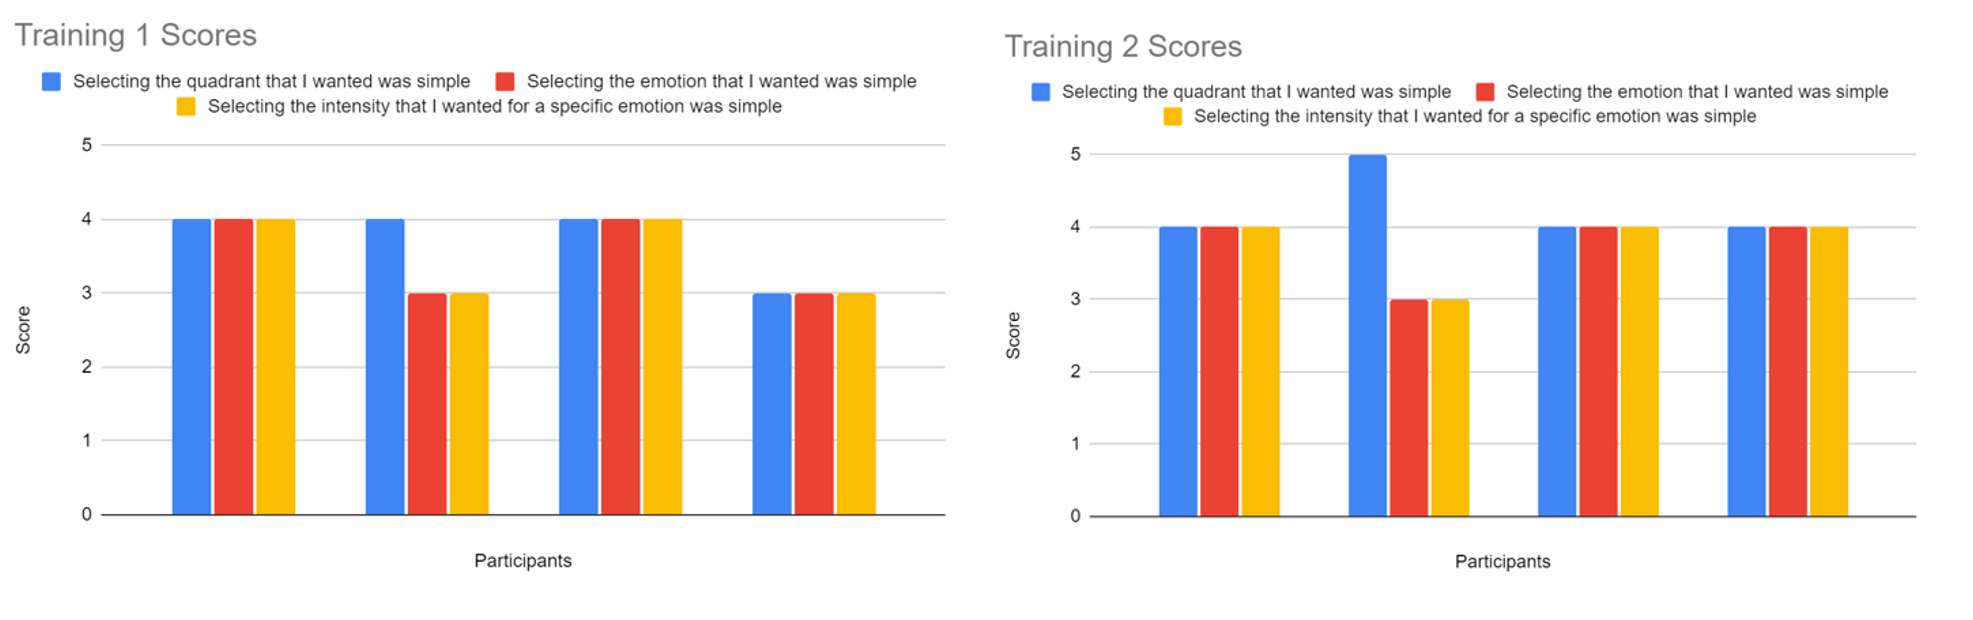
\includegraphics[width=16cm]{img/appendix/usability_condition_A.png}
\centering
\caption{Usability scores for training in condition A (joystick)}\label{fig:usbility_condition_A}
\end{figure}

\begin{figure}[!htb]
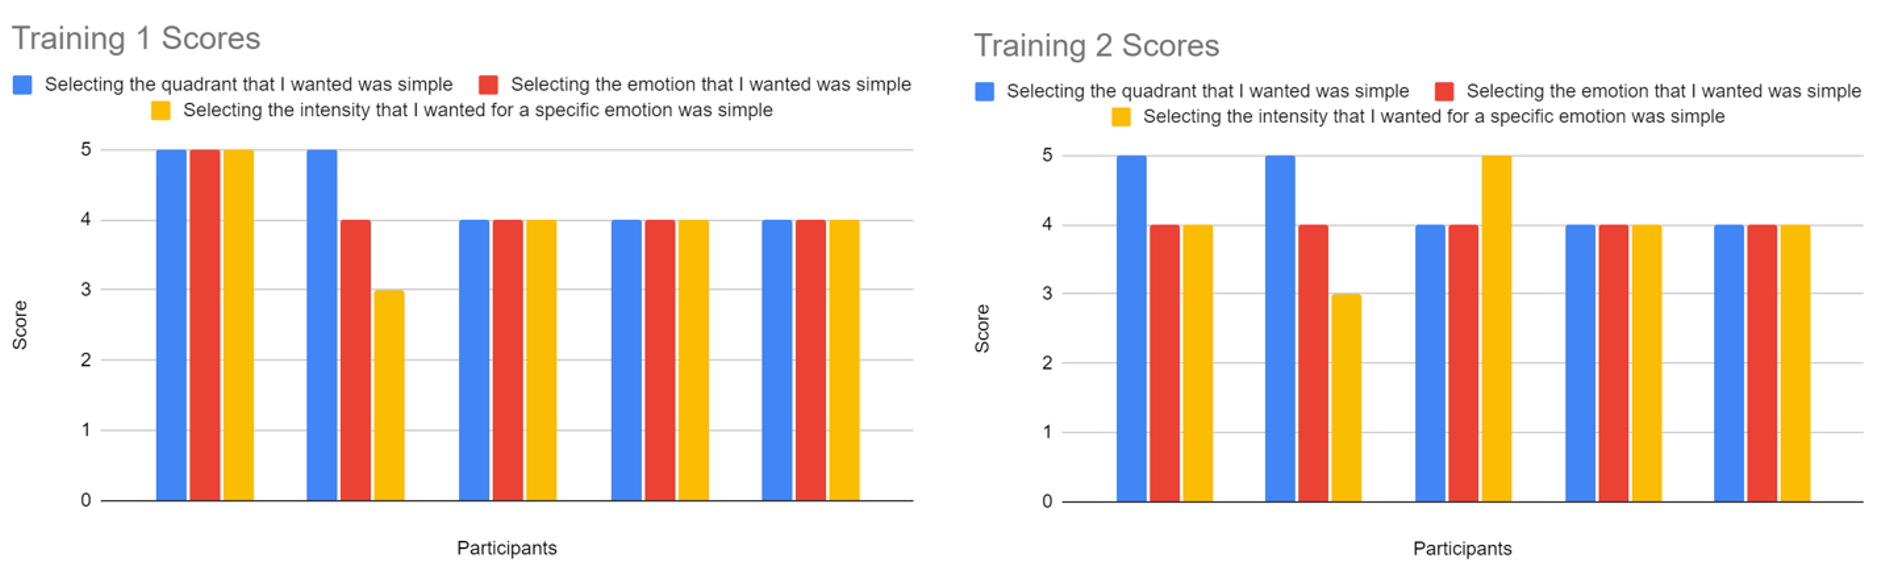
\includegraphics[width=16cm]{img/appendix/usability_condition_B.png}
\centering
\caption{Usability scores for training in condition A (joystick)}\label{fig:usbility_condition_B}
\end{figure}

\begin{table}[!htb]
  \caption{Average usability scores for the two groups.}
  \label{tbl:table_usability__scores}
  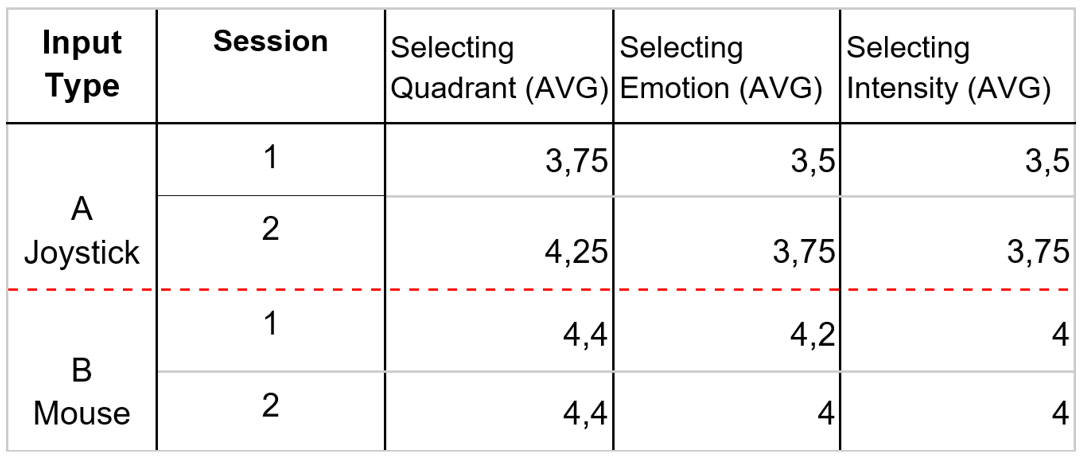
\includegraphics[width=\linewidth]{img/appendix/table_usability_scores.png}
\end{table}

\section{Methods}
\label{sec:appendix_A2}

\subsection{Participants info-graphic}
\label{sec:appendix_A2.1}
\begin{figure}[!htb]
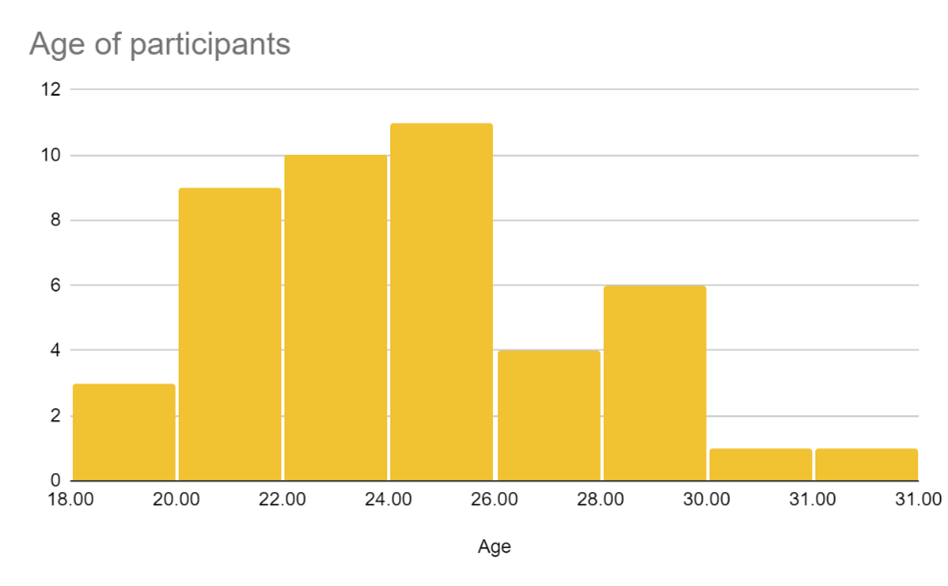
\includegraphics[width=14cm]{img/appendix/age_distribution.png}
\centering
\caption{Usability scores for training in condition A (joystick)}\label{fig:usbility_condition_B}
\end{figure}

\begin{figure}[!htb]
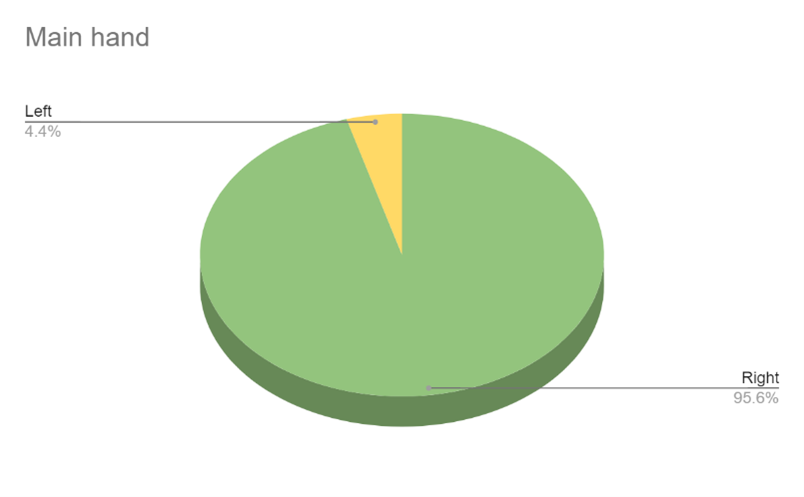
\includegraphics[width=14cm]{img/appendix/right_hand.png}
\centering
\caption{Usability scores for training in condition A (joystick)}\label{fig:usbility_condition_B}
\end{figure}

\subsection{Emotion-Music playlist}
\label{sec:appendix_A2.2}
High Arousal / High Valence (HAHV)
\begin{itemize}
\item  (High arousal, medium positive valence) Excitement- Weapon of choice by Fatboy Slim
\item  (Medium positive arousal, high valence) Happiness - Love Today by Mika
\end{itemize}

High Arousal / High Valence (LAHV)
\begin{itemize}
\item  (Medium negative Arousal, high valence) Satisfaction - Nasty Naughty Boy, by Christina Aguilera
\item 	 (Low arousal, medium positive valence) Relaxation – Amber by 311
\end{itemize}

High Arousal / High Valence (LALV)
\begin{itemize}
\item  (Medium negative arousal, High negative valence) Depression - Last Flowers by Radiohead
\item  (Low arousal, Medium negative valence) Sadness – Hurt by Johnny Cash
\end{itemize}

High Arousal / High Valence (HALV)
\begin{itemize}
\item  (Medium positive arousal, High negative valence) Anger – Threshold by Slayer
\item  (High positive arousal, Medium negative valence) Anxiety - Trapped Under Ice by Believe
\end{itemize}

Other songs were used in the training sessions, but no labelling is provided as their only purpose was 
to teach the users how to use the EA app GUI.
\begin{itemize}
\item  The white stripes - Seven Nation Army
\item  Gary Jules - Mad World
\item  Oren Lavie - Her morning elegance
\item  The Cranberries - Zombie
\item  Maneskin - I wanna be your slave
\item  Rage against the machine - Killing in the name of
\end{itemize}



\section{Intermediate experiments}
\label{sec:appendix_A3}
During the development of the classification pipeline, several intermediate experiments were run to
explore the data, the methodologies, and the different classifiers. The dataset of each subject was 
explored singularly, but only some examples are reported below

\subsection{Subject-dependent experiment with Sequential Features Selection}
\label{sec:appendix_A3.1}

\subsection{Subject-dependent experiment with Top5 features}
\label{sec:appendix_A3.2}

\subsection{Examples of unbalanced datasets}
\label{sec:appendix_A3.3}

\subsection{Subject-independent experiment with Top5 features}
\label{sec:appendix_A3.4}

\subsection{Subject-dependent experiment with "Max Accuracy" scoring strategy}
\label{sec:appendix_A3.5}

\begin{table}[h!]
  \caption{Arousal classification results using "accuracy" as scoring parameter for GridSearch. Learning models are highlighted in blue, over-fitted and under-fitted models are highlighted in yellow and orange, respectively.}
  \label{tbl:max_acc_arousal_results}
  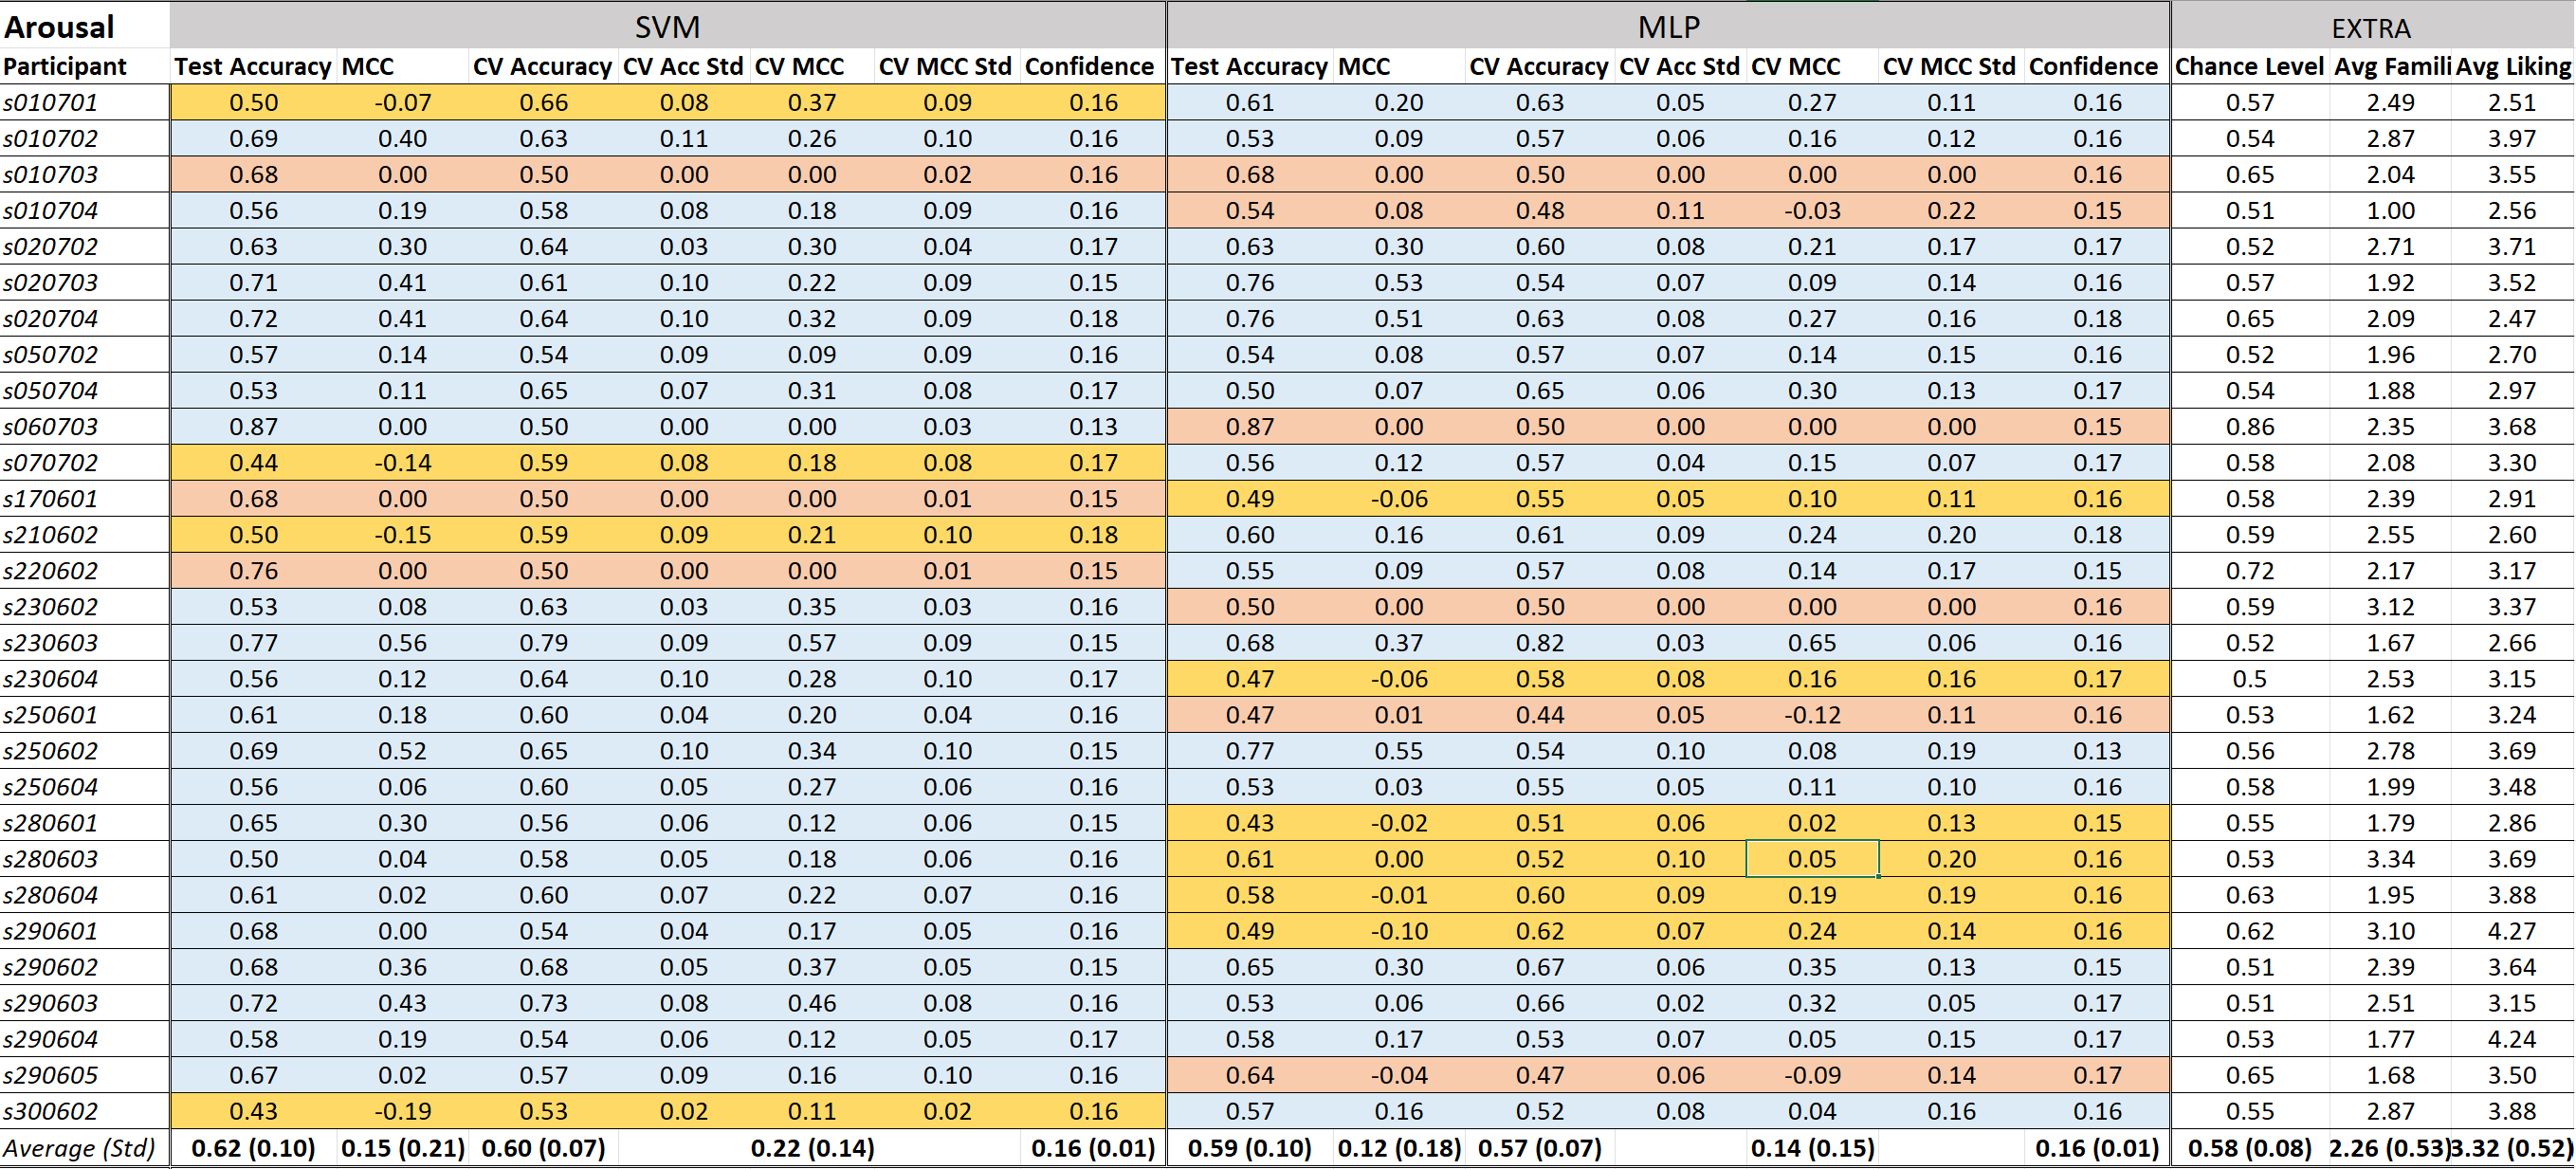
\includegraphics[width=\linewidth]{img/appendix/arousal_max_acc_results.png}
\end{table}

\begin{table}[h!]
  \caption{Valence classification results using "accuracy" as scoring parameter for GridSearch. Learning models are highlighted in blue, over-fitted and under-fitted models are highlighted in yellow and orange, respectively.}
  \label{tbl:max_acc_valence_results}
  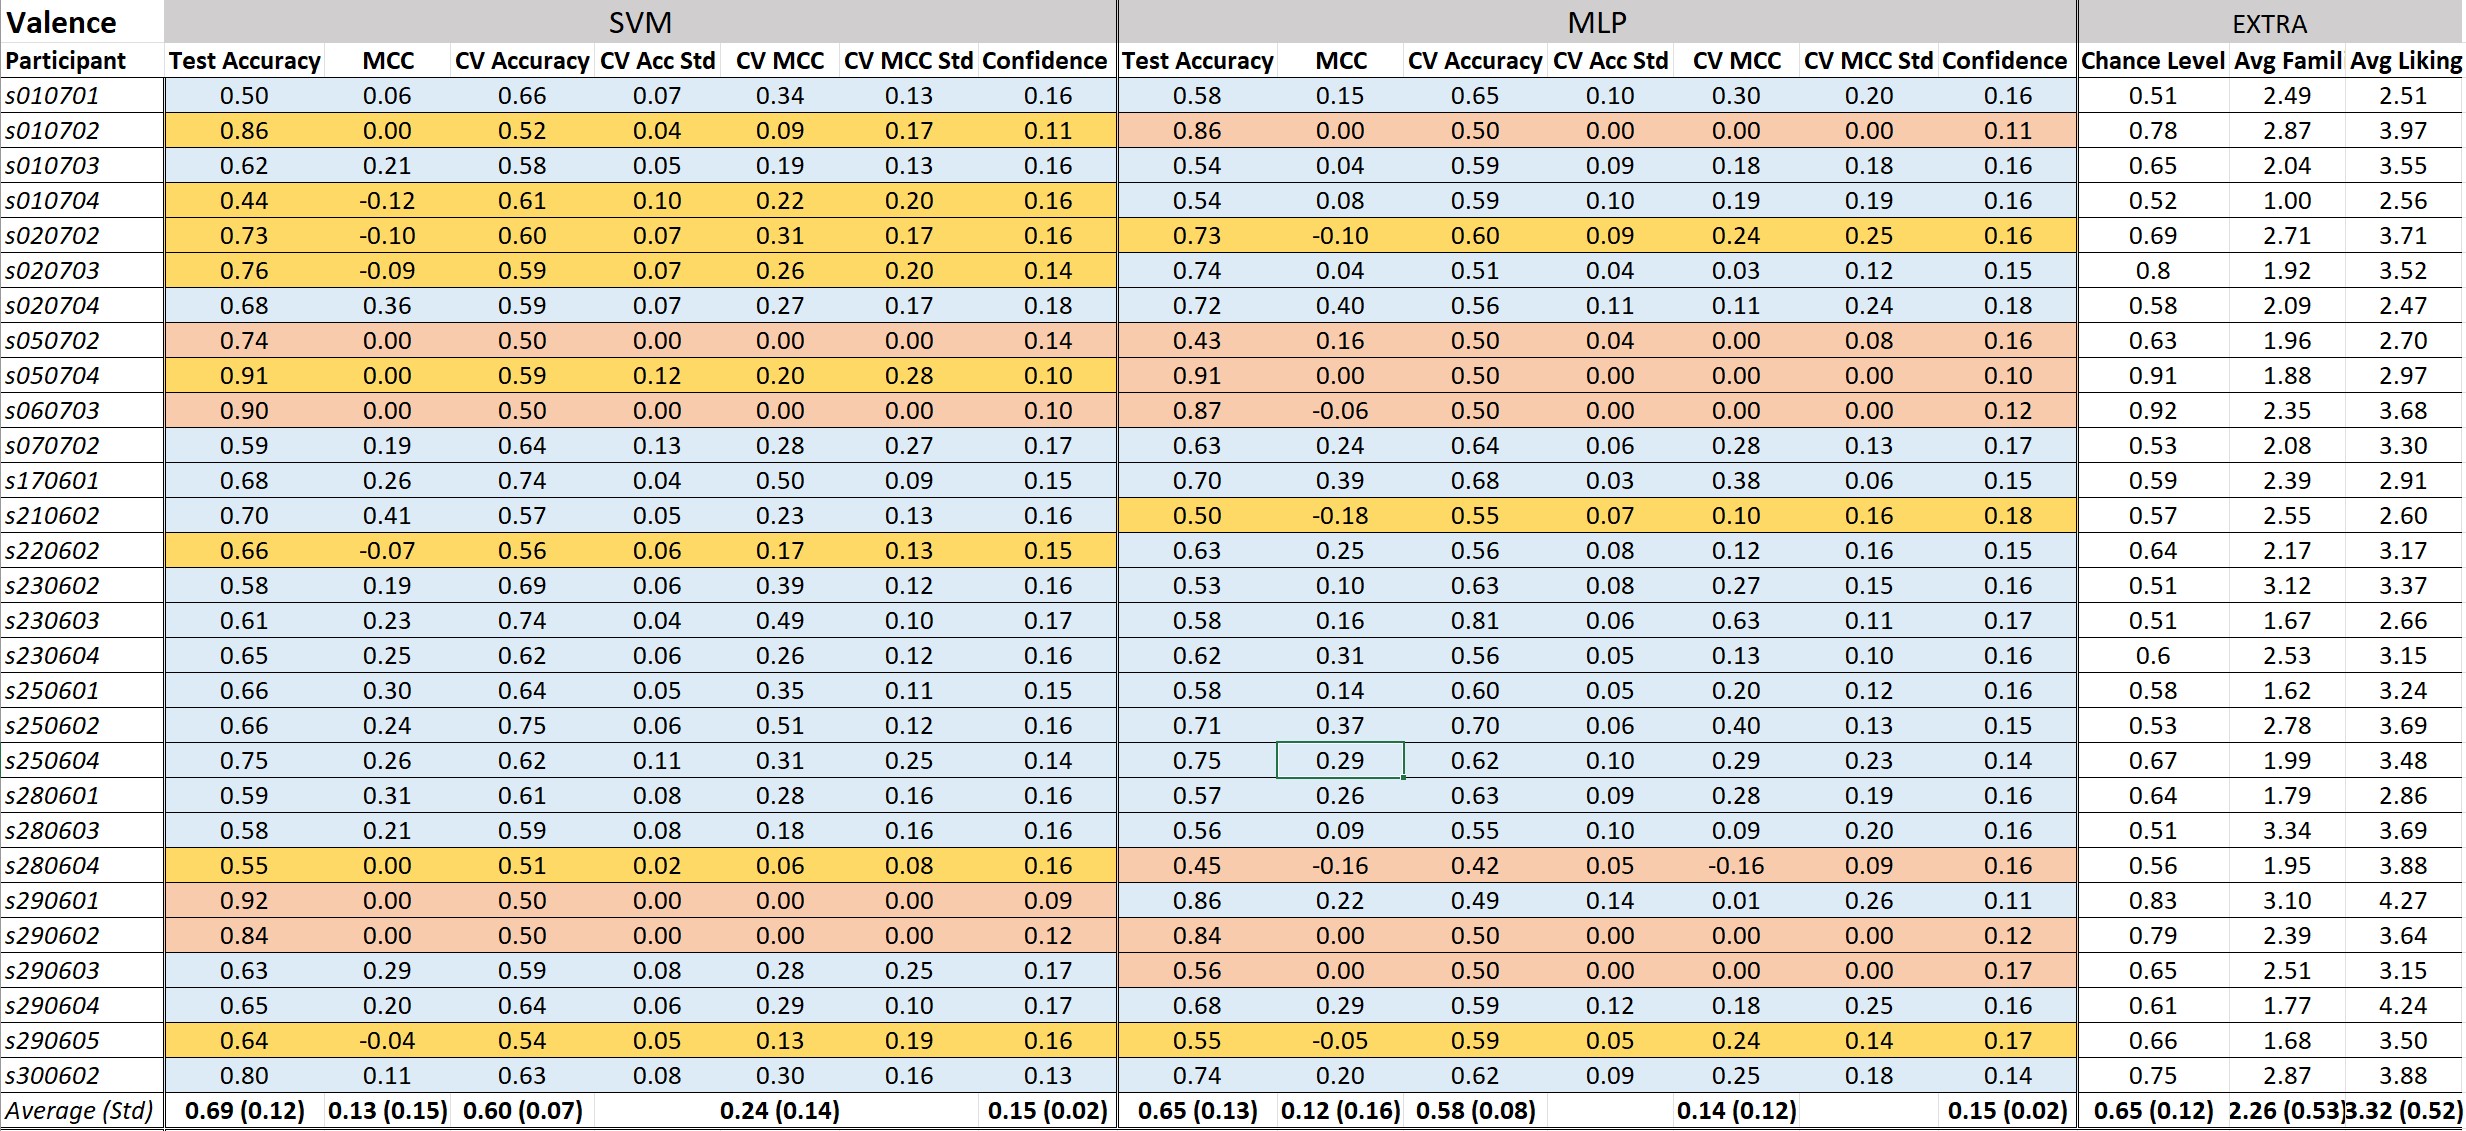
\includegraphics[width=\linewidth]{img/appendix/valence_max_acc_results.png}
\end{table}


\section{Final experiment}
\label{sec:appendix_A4}



